\documentclass{beamer}
\usepackage{amsmath, amssymb, minted}
\usepackage{mathtools}
\usepackage{tikz}
\usetikzlibrary{automata, arrows, positioning, fit, shapes}

\newcommand{\concat}{\mathbin{\cdot}}
\newcommand{\kstar}{{*}}

\DeclarePairedDelimiter\ceil{\lceil}{\rceil}
\DeclarePairedDelimiter\floor{\lfloor}{\rfloor}

\usetheme{Berkeley}
\usecolortheme{mbhs}

\title{Finite Automata and Regular Languages}

\author{Noah Singer, Arman Siddique}
\institute{Montgomery Blair High School Computer Team}

\begin{document}
\pgfdeclarelayer{background}
\pgfsetlayers{background,main}

\begin{frame}
  \titlepage
\end{frame}

\section{Deterministic Finite Automata}

\begin{frame}{DFA}
\begin{definition}[Deterministic Finite Automaton]
A 5-tuple $(Q, \Sigma, \delta, q_0, F)$, where:
\begin{itemize}
\item $Q$ is a finite set of \textit{states} that the DFA may exist in
\item $\Sigma$ is the \textit{alphabet}, a finite set of symbols that the DFA reads in
\item $\delta: Q \times \Sigma \to Q$ is the \textit{transition function}, which maps the current state and the next input symbol to a new state
\item $q_0 \in Q$ is the \textit{start state} of the DFA
\item $F \subseteq Q$ is the set of \textit{accept states} of the DFA
\end{itemize}
\end{definition}
\end{frame}

\begin{frame}{DFA (cont'd.)}
\begin{definition}[DFA Acceptance]
A DFA defined by $(Q, \Sigma, \delta, q_0, F)$ \textit{accepts} a string $w = a_1 a_1 \ldots a_n$ iff there exists some sequence of states $r_0 r_1 \ldots r_n$ in $Q$ where:
\begin{enumerate}
\item $r_0 = q_0$ ($r_0$ is the start state)
\item $r_{i+1} = \delta (r_i, a_{i+1})$, for $i$ between $0$ and $n-1$ ($r_{i+1}$ follows from $r_i$ on input character $a_{i+1}$)
\item $r_n \in F$ ($r_n$ is an accept state)
\end{enumerate}
\end{definition}
\end{frame}

\begin{frame}{Example}
Given a binary string (a string that consists of only ones and zeroes), create a DFA to check whether it contains the substring $001$.
For example, the following binary strings contain the substring $001$:
\begin{itemize}
\item 101\underline{001}
\item 000\underline{001}11111
\item \underline{001}001001
\end{itemize}
\end{frame}

\begin{frame}{Solution}

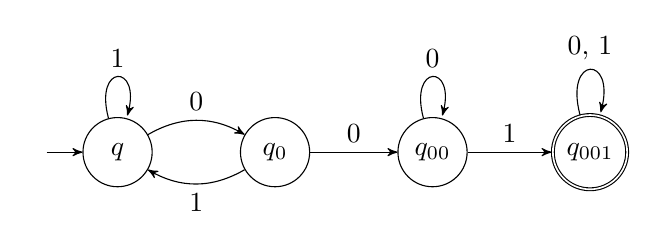
\begin{tikzpicture}[>=stealth',node distance=2cm,on grid,auto]
\node[state,initial,initial text={}] (q) {$q$};
\node[state] (q_0) [right of=q] {$q_0$};
\node[state] (q_00) [right of=q_0] {$q_{00}$};
\node[state,accepting] (q_001) [right of=q_00] {$q_{001}$};
\path[->]
(q)		edge[bend left] node {0} (q_0)
		edge[loop above] node {1} ()
(q_0)	edge node {0} (q_00)
		edge[bend left] node {1} (q)
(q_00)	edge[loop above] node {0} ()
		edge node {1} (q_001)
(q_001)	edge[loop above] node {0, 1} ();
\end{tikzpicture}

\end{frame}

\begin{frame}{Another Example}
Given a binary string, create a DFA to check whether its value is divisible by $3$.
For example, the following binary strings are divisible by $3$:
\begin{itemize}
\item 11 ( = 3)
\item 1001 ( = 9)
\item 10101 ( = 21)
\end{itemize}
\end{frame}

\begin{frame}{Solution}

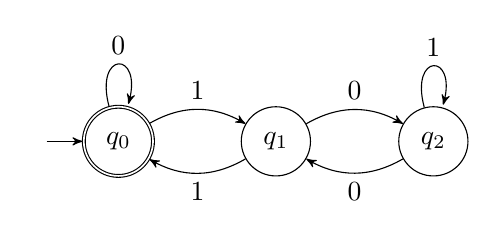
\begin{tikzpicture}[>=stealth',node distance=2cm,on grid,auto]
\node[state,initial,accepting,initial text={}] (q_0) {$q_0$};
\node[state] (q_1) [right of=q_0] {$q_1$};
\node[state] (q_2) [right of=q_1] {$q_2$};
\path[->]
(q_0) edge[loop above] node {0} (q_0)
			edge[bend left] node {1} (q_1)
(q_1) edge[bend left] node {0} (q_2)
			edge[bend left] node {1} (q_0)
(q_2) edge[bend left] node {0} (q_1)
			edge[loop above] node {1} (q_2);
\end{tikzpicture}

Since,
\begin{itemize}
\item $2 \cdot 0 + 0 \equiv 0 \pmod{3}$
\item $2 \cdot 0 + 1 \equiv 1 \pmod{3}$
\item $2 \cdot 1 + 0 \equiv 2 \pmod{3}$
\item $2 \cdot 1 + 1 \equiv 0 \pmod{3}$
\item $2 \cdot 2 + 0 \equiv 1 \pmod{3}$
\item $2 \cdot 2 + 1 \equiv 2 \pmod{3}$
\end{itemize}

\end{frame}

\section{Formal Languages}

\begin{frame}{Languages}
\begin{definition}[Formal Language]
A set $L$, finite or infinite, over some alphabet $\Sigma$, consisting of strings (finite sequences) of symbols in $\Sigma$.
\end{definition}

Examples of languages over the binary alphabet $\Sigma = \{0,1\}$:
\begin{itemize}
	\item $\{0,1,00,11,010,101,111,000,...,110101011,...\}$, the set of all binary palindromes
\item $\{01,0011,000111,00001111\}$, the set of all strings of the form $0^a1^a$
\item $\{10,11,101,111,1011,...\}$, the set of all primes
\end{itemize}

\end{frame}

\begin{frame}{Operations on Languages}
$s^n$ means the string/symbol $s$ repeated $n$ times.

\begin{enumerate}
\item The \textit{union} of two languages $A$ and $B$, $A \cup B$, is defined as $\{q \mid q \in A \vee q \in B\}$.
\item The \textit{concatenation} of two languages $A$ and $B$, $A \cdot B$ or $AB$, is defined as $\{pq \mid p \in A, q \in B\}$.
\item The \textit{Kleene star} of a language $A$, $A*$, is defined as $\{p^n \mid p \in A, n \in \mathbb{N}\}$.
\end{enumerate}

Some examples:
\begin{itemize}
\item $\{aba\} \cup \{bab\} = \{aba, bab\}$
\item $\{aba, bab\} \concat \{b\} = \{abab, babb\}$
\item $\{aba\} \kstar = \{\epsilon, aba, abaaba, abaabaaba, \ldots\}$
\end{itemize}
\end{frame}

\section{Regular Languages}

\begin{frame}{Regular Languages}
\begin{definition}[Regular Language]
The \textit{family} of regular languages $R$ is defined as the \textit{closure} of the family $\{\varnothing, \{\epsilon\}, \{s_0\}, \{s_1\}, ...\}$ for $s_i$ in $\Sigma$ under the operations of union, concatenation, and Kleene star.
\end{definition}

Motivation: \textit{Regular languages are exactly the set of strings recognizable by finite automata}.
\end{frame}

\begin{frame}{Regular Expressions}
\begin{itemize}
\item An arithmetic expression evaluates to a \textit{number}
\item A regular expression evaluates to a \textit{regular language}
\item Shorthand for representing a regular language used often in programming and scripting
\item Regular expressions have operands and operators
\item Operands are regular expressions
\item Operators combine, modify, or manipulate regular expressions
\end{itemize}
\end{frame}

\begin{frame}{Syntax}
In the following, $\alpha$ and $\beta$ represent two regular expressions, and $A$ and $B$ the regular languages the evaluate to, respectively.

\vspace{0.1in}
\begin{tabular}{c|cc}
Expression & Set Theory & Meaning \\
\hline
$\alpha \mid \beta$ & $A \cup B$ & Either $A$ or $B$ \\
$\alpha \beta$ & $A \concat B$ & $A$ followed by $B$ \\
$\alpha \kstar$ & $A \kstar$ & Zero or more copies of $A$ \\
$\alpha+$ & $A \concat A \kstar$ & One or more copies of $A$ \\
$\alpha?$ & $A \cup \{\epsilon\}$ & Zero or one copy of $A$ \\
\end{tabular}
\end{frame}

\section{Non-Deterministic Finite Automata}

\begin{frame}{NFA Intuition}
\begin{itemize}
	\item Like a DFA, but it can exist in multiple states simultaneously (can allow multiple transitions from the same state with the same symbol to different states)
    \item \textit{Nondeterministic} since we can be in multiple states at once
    \item $\epsilon$-transitions allow transitions between states while accepting no input
    \item All DFAs are NFAs
    \begin{itemize}
    	\item Eventually we'll show that all NFAs can be converted to DFAs
    \end{itemize}
    \item Certain properties of DFAs can be proved more easily with NFAs
\end{itemize}
\end{frame}

\begin{frame}{NFA}
\begin{definition}[Nondeterministic Finite Automaton]
A 5-tuple $(Q, \Sigma, \delta, q_0, F)$, where:
\begin{itemize}
\item $Q$ is a finite set of \textit{states} that the NFA may exist in
\item $\Sigma$ is the \textit{alphabet}, a finite set of symbols that the NFA reads in
\item $\Delta: Q \times (\Sigma \cup \{\epsilon\}) \to \mathcal{P}(Q)$ is the \textit{transition function}, which maps the current state and the next input symbol or $\epsilon$ to a new subset of states
\item $q_0 \in Q$ is the \textit{start state} of the NFA
\item $F \subseteq Q$ is the set of \textit{accept states} of the NFA
\end{itemize}
\end{definition}
\end{frame}

\begin{frame}{NFA (cont'd.)}
\begin{definition}[$\epsilon$-closure]
The $\epsilon$-closure of some state $q \in Q$, denoted $E(q)$, is defined of the set of states $p$ such that there exists some sequence of states $q_1 q_2 ... q_k$ such that:

\begin{enumerate}
\item $q_1 = q$
\item $q_2 = \Delta(q_1, \epsilon)$
\item $q_k = p$	
\end{enumerate}
\end{definition}
\end{frame}

\begin{frame}{NFA (cont'd.)}
\begin{definition}[NFA Acceptance]
An NFA defined by $(Q, \Sigma, \Delta, q_0, F)$ accepts a string $w = a_1 a_1 \ldots a_n$ iff there exists some sequence of states $r_0 r_1 \ldots r_n$ in $Q$ where:

\begin{enumerate}
\item $r_0 = E(q_0)$
\item $r_{i+1} = E(\Delta (r_i, a_{i+1}))$, for $i$ between $0$ and $n-1$
\item $r_n \in F$
\end{enumerate}
\end{definition}
\end{frame}

\begin{frame}{Problem}
Given a string consisting only of zeroes (a unary alphabet), create an NFA to check whether its length is a multiple of two or three.
\end{frame}

\begin{frame}{Solution}
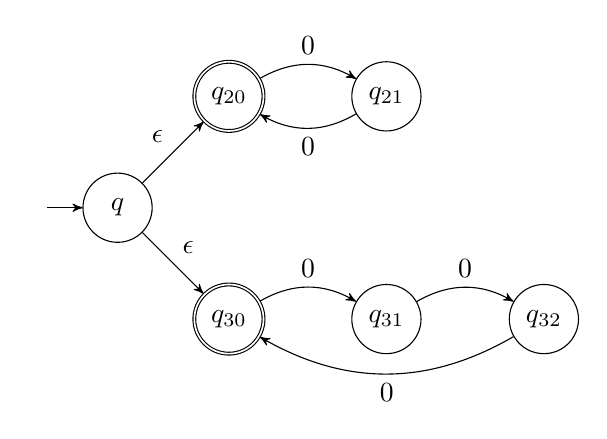
\begin{tikzpicture}[>=stealth',node distance=2cm,on grid,auto]
\node[state,initial,initial text={}] (q) {$q$};
\node[state,accepting] (q_20) [above right of=q] {$q_{20}$};
\node[state] (q_21) [right of=q_20] {$q_{21}$};
\node[state,accepting] (q_30) [below right of=q] {$q_{30}$};
\node[state] (q_31) [right of=q_30] {$q_{31}$};
\node[state] (q_32) [right of=q_31] {$q_{32}$};
\path[->]
(q)	edge node {$\epsilon$} (q_20)
		edge node {$\epsilon$} (q_30)
(q_20) edge[bend left] node {0} (q_21)
(q_21) edge[bend left] node {0} (q_20)
(q_30) edge[bend left] node {0} (q_31)
(q_31) edge[bend left] node {0} (q_32)
(q_32) edge[bend left] node {0} (q_30);
\end{tikzpicture}
\\
\vspace{.1in}
The idea of $\epsilon$ is helpful in expressing the ``or''.  It is non-obvious how to solve this problem with a DFA.
\end{frame}


\begin{frame}{Problem}
Create an NFA to determine whether a binary string ends with the string 0001.
\end{frame}

\begin{frame}{Solution}
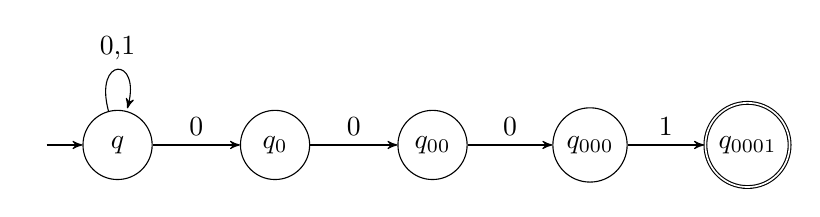
\begin{tikzpicture}[>=stealth',node distance=2cm,on grid,auto]
\node[state,initial,initial text={}] (q) {$q$};
\node[state] (q_0) [right of=q] {$q_0$};
\node[state] (q_00) [right of=q_0] {$q_{00}$};
\node[state] (q_000) [right of=q_00] {$q_{000}$};
\node[state,accepting] (q_0001) [right of=q_000] {$q_{0001}$};
\path[->]
(q)	edge[loop above] node {0,1} (q)
		edge node {0} (q_0)
(q_0) edge node {0} (q_00)
(q_00) edge node {0} (q_000)
(q_000) edge node {1} (q_0001);
\end{tikzpicture}
\\
\vspace{.1in}
Again, it is non-obvious how to do this in a strictly deterministic manner.
\end{frame}


\begin{frame}{Thompson's Construction}
\begin{theorem}[Thompson's Construction]
All regular languages may be \textit{recognized} by non-deterministic finite automata.
\end{theorem}

Proof sketch: Let $N(A)$ denote the NFA corresponding to regular language $A$.  We show that $N(\{\epsilon\})$ and $N(\{x\})$ for $x$ in $\Sigma$ exist.  We then show how to construct the NFA under each regular language operation and therefore our proof is complete by closure.
\end{frame}

\begin{frame}{Thompson's Construction: Basics}
The NFA for $x \in \Sigma \cup \{\epsilon\}$ is: \\
\vspace{0.1in}

\begin{center}
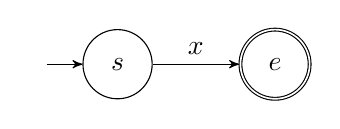
\begin{tikzpicture}[>=stealth',node distance=2cm,on grid,auto]
\node[state,initial,initial text={}] (s) {$s$};
\node[state,accepting] (e) [right of= s] {$e$};
\path[->]
(s)	edge node {$x$} (e);
\end{tikzpicture}
\end{center}
\end{frame}

\begin{frame}{Thompson's Construction: Union}
The NFA for $A \cup B$, where $A$ and $B$ are regular, is: \\
\vspace{0.1in}

\begin{center}
\begin{tikzpicture}[>=stealth',node distance=2cm,on grid,auto]
\node[state,initial,initial text={}] (s) {$s$};
\node[state,fill=green!20] (s_A) [above right of=s] {$s_A$};
\node[state,fill=red!20] (s_B) [below right of=s] {$s_B$};
\node[state,fill=green!20] (e_A) [right = 2.5 of s_A] {$e_A$};
\node[state,fill=red!20] (e_B) [right = 2.5 of s_B] {$e_B$};
\node[state,accepting] (e) [below right of=e_A] {$e$};
\path[->]
(s)	edge node {$\epsilon$} (s_A)
		edge node {$\epsilon$} (s_B)
(e_A)	edge node {$\epsilon$} (e)
(e_B)	edge node {$\epsilon$} (e);

\begin{pgfonlayer}{background}
\node[ellipse,draw=green!20,fill=green!10,fit=(s_A) (e_A)](FIt2) {$N(A)$};
\node[ellipse,fill=red!20,fill=red!10,fit=(s_B) (e_B)](FIt2) {$N(B)$};
\end{pgfonlayer}
\end{tikzpicture}
\end{center}
\end{frame}

\begin{frame}{Thompson's Construction: Concatenation}
The NFA for $A \concat B$, where $A$ and $B$ are regular, is: \\
\vspace{0.1in}

\begin{center}
\begin{tikzpicture}[>=stealth',node distance=2cm,on grid,auto]
\node[state,initial,initial text={},fill=green!20] (s_A) {$s_A$};
\node[state,fill=green!20] (e_A) [right = 2.5 of s_A] {$e_A$};
\node[state,fill=red!20] (s_B) [below of= s_A] {$s_B$};
\node[state,accepting,fill=red!20] (e_B) [right = 2.5 of s_B] {$e_B$};
\path[->]
(e_A) edge node {$\epsilon$} (s_B);

\begin{pgfonlayer}{background}
\node[ellipse,draw=green!20,fill=green!10,fit=(s_A) (e_A)](FIt2) {$N(A)$};
\node[ellipse,fill=red!20,fill=red!10,fit=(s_B) (e_B)](FIt2) {$N(B)$};
\end{pgfonlayer}
\end{tikzpicture}
\end{center}
\end{frame}

\begin{frame}{Thompson's Construction: Kleene Star}
The NFA for $A \kstar$, where $A$ is regular, is: \\
\vspace{0.1in}

\begin{center}
\begin{tikzpicture}[>=stealth',node distance=2cm,on grid,auto]
\node[state,initial,initial text={}] (s) {$s$};
\node[state,fill=green!20] (s_A) [right of= s] {$s_A$};
\node[state,fill=green!20] (e_A) [right = 2.5 of s_A] {$e_A$};
\node[state,accepting] (e) [right of = e_A] {$e$};
\path[->]
(s) edge node {$\epsilon$} (s_A)
	edge [bend right=45] node {$\epsilon$} (e)
(e_A) 	edge node {$\epsilon$} (e)
		edge [bend right=90] node {$\epsilon$} (s_A);

\begin{pgfonlayer}{background}
\node[ellipse,draw=green!20,fill=green!10,fit=(s_A) (e_A)](FIt2) {$N(A)$};
\end{pgfonlayer}
\end{tikzpicture}
\end{center}
\end{frame}


\begin{frame}{Powerset Construction (Rabin-Scott)}
\begin{theorem}[Powerset Construction]
Any non-deterministic finite automaton with $n$ states can be converted into an equivalent deterministic finite automaton with up to $2^n$ states. 
\end{theorem}
Intuition:
\begin{itemize}
\item A DFA needs to keep track of a \textit{single} state at a times
\item An NFA needs to keep track of \textit{many} states at a times
\item Have each DFA state correspond to the \textit{set of states} that the NFA is currently in
\end{itemize}
\end{frame}

\begin{frame}{Proof Sketch}
If the NFA has $\epsilon$-transitions, we can consolidate the states by taking $\epsilon$-closures until there are no more $\epsilon$-transitions.  Therefore, we assume that it has no $\epsilon$-transitions.

For any NFA $N = (Q_N, \Sigma_N, \Delta_N, q_{0N}, F_N)$, we will specify an equivalent DFA $M$ as follows:
\begin{itemize}
\item $Q_M = \mathcal{P}(Q_N)$
\item $\Sigma_M = \Sigma_N$
\item $q_{0M} = \{q_{0N}\}$
\item $\delta_M(S \in Q_M, x \in \Sigma) = \bigcup\limits_{x \in S} \Delta (q, x)$
\item $F_M = \{ \exists q (q \in S \wedge q \in F_N) \mid S \in \mathcal{P}(Q_N)\}$
\end{itemize}
\end{frame}

\begin{frame}{Kleene's Algorithm}
\begin{theorem}[Kleene's Algorithm]
The language recognized by any given deterministic finite automaton is regular.
\end{theorem}

Let the states of the DFA be $Q=\{q_0,q_1,\ldots,q_n\}$, the accept states be $F$, the alphabet be $\Sigma$, and the start state be $q_0$.  We use $R^k_{ij}$ to denote the language of strings that take the DFA from state $q_i$ to state $q_j$ while only passing through states with numbers less than or equal to $k$ (not including the starting and stopping states). 
\end{frame}

\begin{frame}{Proof Sketch}
For $k=-1$, $R^{-1}_{ij}$ =
\[ \begin{cases} 
      \{x \in \Sigma \mid \delta(q_i,x) = q_j\} & i \neq j \\
      \{x \in \Sigma \mid \delta(q_i,x) = q_j\} \cup \epsilon & i = j
   \end{cases}
\]

For some arbitrary $0 \leq k \leq n$, $R^k_{ij}$ = $$(R^{k-1}_{ik} \concat R^{k-1}_{kk} \kstar \concat R^{k-1}_{kj}) \cup R^{k-1}_{ij}$$.

The regular language that represents the entire DFA is $$\bigcup_{q_i \in F} R^n_{0i}$$.
\end{frame}

\begin{frame}{Conclusion}
We have proven the following:

\begin{enumerate}
\item Every regular language can be recognized by an NFA.
\item Every NFA can be converted into a DFA.
\item Every DFA recognizes a regular language.
\end{enumerate}

\begin{center}
\Huge \textbf{DFA = NFA = RL}
\end{center}
\end{frame}

\section{Pumping Lemma}

\begin{frame}{Pumping Lemma}
\begin{theorem}[Pumping Lemma]
For any regular language $L$, there exists some integer $p \geq 1$that for every string $w$ where $|w| \geq p$, there are three strings $x,y,z$ where:
\begin{enumerate}
\item $|y| > 0$
\item $|xy| \leq p$
\item $\forall i \geq 0$, $xy^iz \in L$
\end{enumerate}
\end{theorem}
\end{frame}

\begin{frame}[fragile]{Pumping Lemma Visualization}
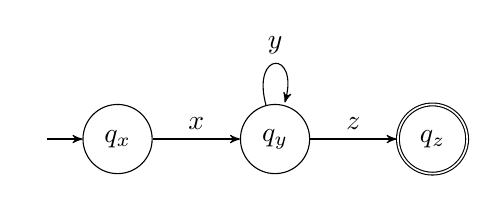
\begin{tikzpicture}[>=stealth',node distance=2cm,on grid,auto]
\node[state,initial,initial text={}] (q_x) {$q_x$};
\node[state] (q_y) [right of=q_x] {$q_{y}$};
\node[state,accepting] (q_z) [right of=q_y] {$q_{z}$};
\path[->]
(q_x) edge node {$x$} (q_y)
(q_y) edge[loop above] node {$y$} (q_y)
(q_y) edge node {$z$} (q_z);
\end{tikzpicture}

We say that the string $y$ can be ``pumped''.
\end{frame}

\begin{frame}{Proof of the Pumping Lemma}
For some regular language $L$, there must exist a DFA $M$ which recognizes it.  Let $p$ be the number of states of $M$.  Let $w \in L$ be a string such that $|w| \geq p$.  Then let the sequence of the start state and first $p$ states that $w$ takes through $M$ be labeled $q_0, q_1, q_2, \ldots, q_p$.  By the pigeonhole principle, since this sequence has $p+1$ states in it, one state must have been visited twice.  Let $q_s$ denote this state.  The section of $w$ that takes $M$ from the first occurence of state $q_s$ to the second is then $y$.  Clearly, $|y| > 0$.  $|xy| \leq p$ since $s \leq p$.  The string $y$ can also be repeated any number of times.  The conditions of the theorem are therefore satisfied.
\end{frame}

\begin{frame}{Applications of the Pumping Lemma}
Let $L = \{a^n b^n \mid n \geq 0\}$, the set of strings consisting of $n$ $a$'s followed by $n$ $b$'s.  Let $p$ be the integer given by the lemma.  Then consider the string $a^p b^p \in L$.  According to the pumping lemma, $a^p b^p = xyz$, with $|xy| \leq p, |y| > 0$.  But since $|xy| \leq p$, then $x$ and $y$ may only contain the letter $a$, and $y$ is non-empty.  We can pump $y$ by repeating it as many times as we want.  When we do this, we are only adding more $a$'s to the string.  This is clearly impossible, since there must be the same number of $a$'s and $b$'s for all words in $L$.  So $L$ is not regular by contradiction.
\end{frame}

\end{document}